	\begin{tikzpicture}

		% A letra "g" e sua caixa
		\node (g) %at (2,0)
			{\raisebox{-1cm}{%
				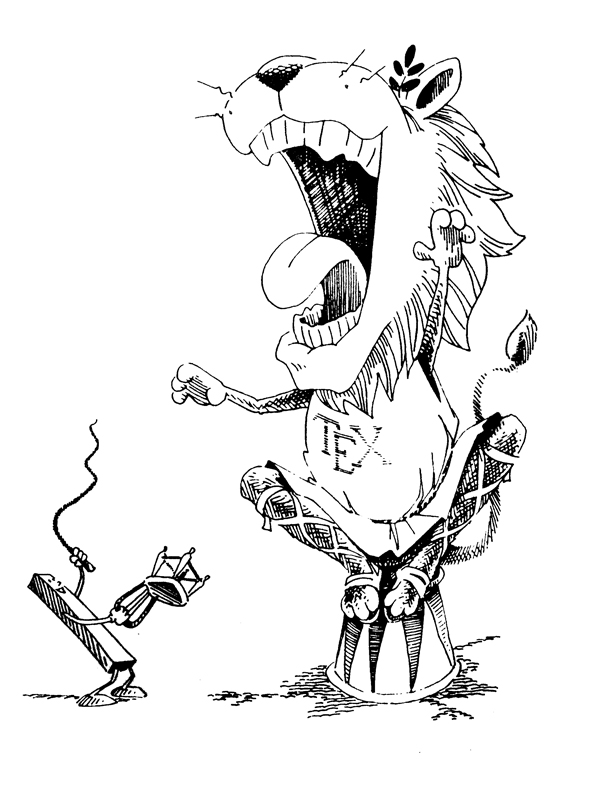
\includegraphics[width=\textwidth]{controlling_TeX_800x600}%
			}};
		%\draw [very thick,red!80] (g.south west) rectangle (g.north east);
		\draw [box] (g.south west) rectangle (g.north east);
		
		%\coordinate (base line left)  at ($(g.base west) - (5mm,0)$);
		%\coordinate (base line right) at ($(g.base east) + (5mm,0)$);
		
		% A linha-base
		%\draw [thick,blue] (base line left) -- (base line right);
		\draw [baseline] ($(g.base west) - (0.1\textwidth,0)$) --
										 ($(g.base east) + (0.1\textwidth,0)$);
				
		% A flecha e o rótulo "Linha-base"
		%\draw [<-,gray!50] ($(base line right) + (1mm,0)$) -- ++(5mm,0)
		%	node [inner sep=0mm, label=right:\textcolor{gray!50}{Linha-base}] {};
		
		% O ponto-de-referência
		\fill [black] (g.base west) circle (3pt);
		
		% Flecha da altura
		%\draw [<->,gray!50] ($ (g.base west) + (-3mm,+0.5mm) $) --
		%            ($ (g.north west) + (-3mm,0) $);
		
		% Flecha da profundidade
		%\draw [<->,gray!50] ($ (g.south west) + (-3mm,0) $) -- 
		%            ($ (g.base west) + (-3mm,-0.5mm) $);

		% Flecha da largura
		%\draw [<->,gray!50] ($ (g.north west) + (0,3mm) $) --
		%            ($ (g.north east) + (0,3mm) $);
		           
		% Flecha da altura total
		%\draw [<->,gray!50] ($ (g.south east) + (3mm,0) $) --
		%            ($ (g.north east) + (3mm,0) $);
		
		% Rótulo "Altura"
		%\node [inner sep=3mm, label=left:\textcolor{gray!50}{Altura}]
	  %		at ($ (g.base west)  ! 0.5 ! (g.north west) $) {};
		
		% Rótulo "Profundidade"
		%\node [inner sep=3mm, label=left:\textcolor{gray!50}{Prof.}]
		%	at ($ (g.base west)  ! 0.5 ! (g.south west) $) {};
		
		% Rótulo "Largura"
		%\node [inner sep=3mm, label=above:\textcolor{gray!50}{Largura}]
		%	at ($ (g.north west) ! 0.5 ! (g.north east) $) {};
		
		% Rótulo "Altura total"
		%\node [inner sep=3mm, label=right:\textcolor{gray!50}{Altura total}]
		%	at ($ (g.base east)  ! 0.5 ! (g.north east) $) {};
		
		% Flecha e rótulo "Ponto-de-referência"
		%\draw [<-,gray!50] ($(g.base west) + (3pt,-3pt)$) -- ++(3mm,-3mm) --
		 %++(0mm,-1cm)
			%node [circle,inner sep=0mm,label=below:\textcolor{gray!50}{Ponto-de-%
			%referência}] {};		
	\end{tikzpicture}